\documentclass{handout}

\SetInstructor{Lt Col James Phillips}
\SetCourseTitle{ECE231: Electrical Circuits and Systems I}
\SetSemester{Spring 2016}
\SetHandoutTitle{Lecture 33:Filters I -- Transfer Functions}

%\SetDueDate{1 Jan 2016}
%\ShowAllBlanks

\showsoln \setsolncolor{red}

\begin{document}
\maketitle

\textbf{Upcoming events}
\begin{enumerate}
\item Problem Set \# 7 due Lesson 37
\item Quiz \# 6 Lesson 37
\item GR \# 3 Lesson 38
\end{enumerate}

\textbf{OBJECTIVES:}
\begin{enumerate}
\item Understand how to calculate and interpret magnitude and phase responses
\item Understand the concept of a transfer function and its frequency dependence
\end{enumerate}

\textbf{READING}
\begin{description}
\item [Required]:
Filters Handout (Available on Sharepoint), pgs 1-13
\item [Optional]: 
\end{description}

\textbf{HOMEWORK}
\begin{description}
\item [Required problems]: 
\item [Recommended textbook problems]: 1--1, 1--2, 1--3 (Handout)
\end{description}

\section{Introduction}
Throughout the last 4 lessons, we have been working with complex numbers to solve {\em single frequency sinusoidal}, steady state circuits.  During this lesson, we are going to start allowing frequency, $\omega$, to vary.  In order to look a the behavior of a circuit as $\omega$ varies, we will learn to build magnitude and phase plots.  Since we are no longer fixing $\omega$, we will not calculate impedances and solve circutis in the same manner.

\section{Magnitude Plots}
Since we have been looking at circuits with a single fixed frequency, our complex numbers (whether voltage, current or impedance) have had a fixed real part and a fixed imaginary part. As stated above, we are now going to allow $\omega$ to vary, so we will write our complex numbers in one of the forms below:
\soln{1.5in}{
 \[
 K[R+j\omega]
 \]
 \[
 K\left[R+\frac{1}{j\omega}\right]
 \]
 }
 The reason for this will hopefully be obvious later.
 
 Let's look at a couple of impedances to convice ourselves that write any complex number in this form; this will help us later when we want to write transfer functions in standard form; \textbf{our standard form will always have $j$ and $\omega$ together and the coefficient on highest order of $j\omega$ will always be 1}.  Let $Z_L = R_L+j\omega L$ and $Z_C = R_C-\frac{j}{\omega C}$; write both of these impedances in the form $K[R+j\omega]$:

\soln{4in}{
For $Z_L$, let $K = L$ therfore:
\[
Z_L =  L[\frac{R}{L} +j\omega]
\]

$Z_C$ is a little harder.... We first want o rewrite $Z_C$ to put the $j$ and the $\omega$ back together
\[
Z_C = R_C+\frac{1}{j\omega C}
\]
Next, factor out a $\frac{1}{C}$
\[
Z_C = \frac{1}{C}\left[R_CC+\frac{1}{j\omega}\right]
\]
}

Now that we know how to right complex numbers in this {\em standard form} (we really over use that term), lets solve for the magnitude of a couple of examples and plot that magnitude vs fequency:

First lets find the magnitude of $20+j\omega$:
\soln{1.5in}{
\[
|100 + j\omega|=\sqrt{100^2+\omega^2} = \sqrt{10,000 +\omega^2}
\]
}

We can use MATLAB to plot this:
\begin{figure} [h!]
\centering
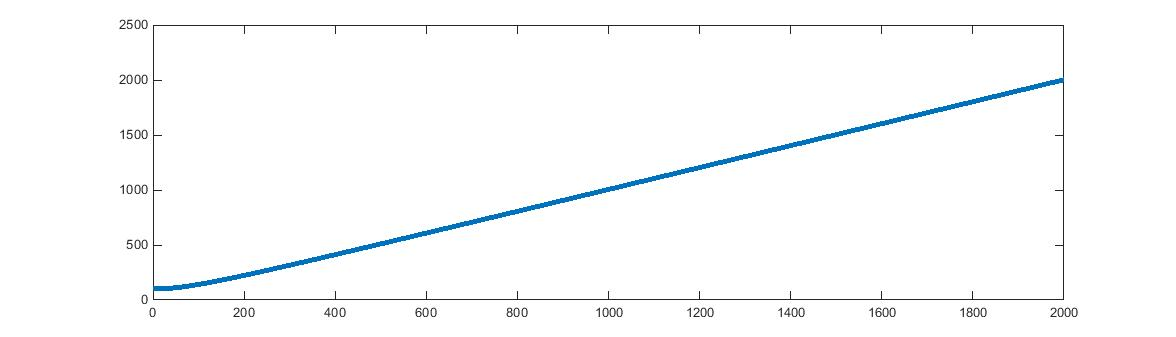
\includegraphics[width=1\textwidth]{MagResponse1.jpg}
\caption{A simple magnitude respsonse}
\label{fig: MagResponse1}
\end{figure}

\newpage
\clearpage
\pagebreak

Let's add some complexity by going onto an example from the reading.  Lets do a magnitude plot for: $\frac{200}{j\omega +50}$

\soln{2in}{
Start by calculating the magnitude as a function of $\omega$:
\[
\left|\frac{200}{j\omega +50}\right|=\frac{|200|}{|j\omega +50|}=\frac{200}{\sqrt{50^2 + \omega^2}}=\frac{200}{\sqrt{2500 + \omega^2}}
\]
}
We can plot this in MATLAB as well:

\begin{figure} [h!]
\centering
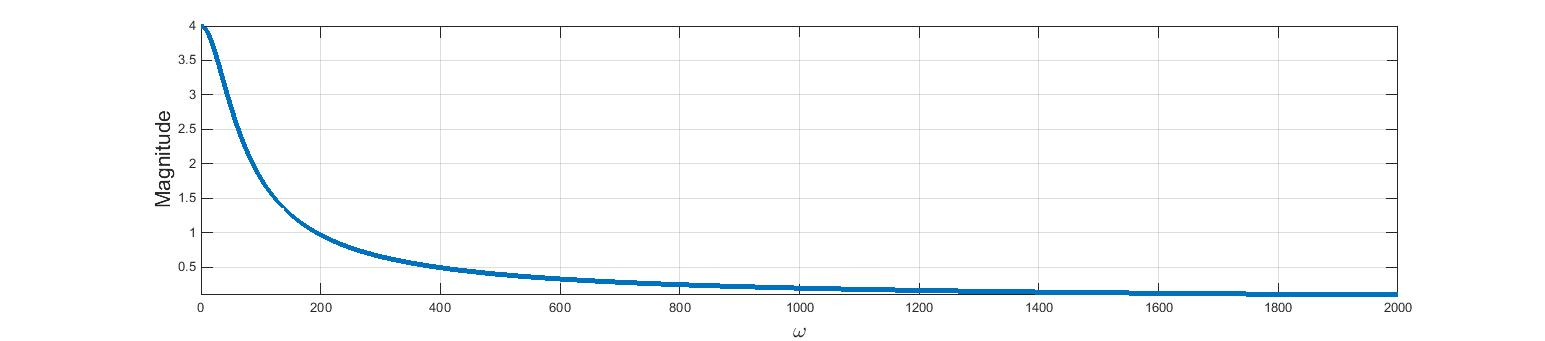
\includegraphics[width=1\textwidth]{MagResponse2.jpg}
\caption{A slightly more complex magnitude respsonse}
\label{fig: MagResponse2}
\end{figure}

For the next several lessons we need to get in the habit of using semi-log plots.  This will make some of the frequency dependent behavior easier to interpret.  Tha magnitude response above replotted on a semilog scale would look like:
\begin{figure} [h!]
\centering
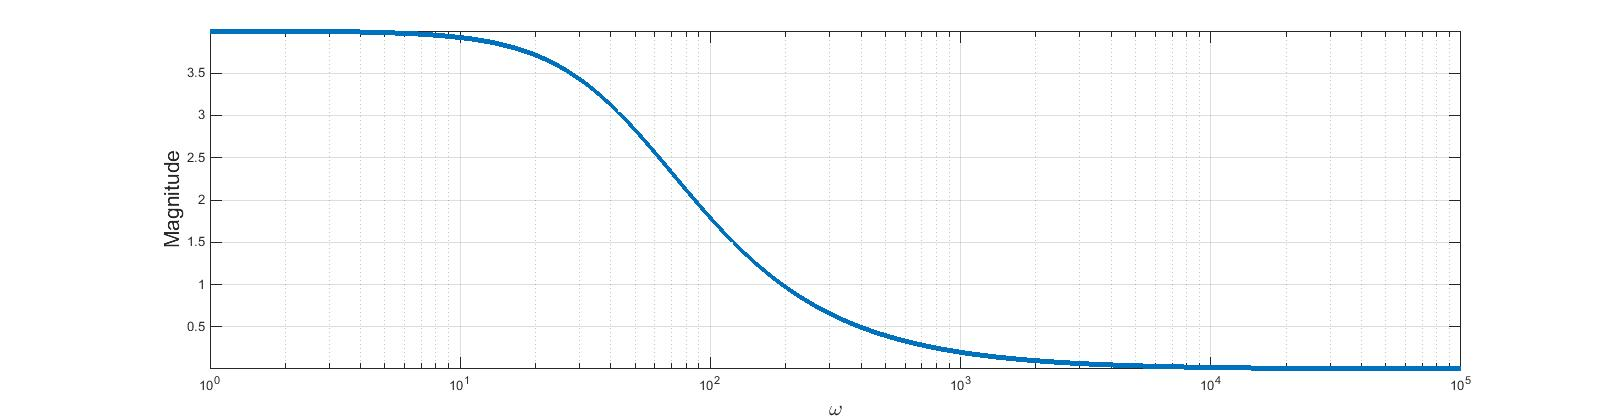
\includegraphics[width=1\textwidth]{MagResponse3.jpg}
\caption{Magnitude response plotted on a semilog (x) scale}
\label{fig: MagResponse3}
\end{figure}

If you look closely you will see these plots contain the exact some information. 
\newpage
\clearpage
\pagebreak
\section{Phase Response}
Remember complex numbers have both magnitude (discussed above) and phase.  If we look at the complex number $K+j\omega$, the phase is:
\soln{1in}{
\[
\theta=\tan^{-1}\left(\frac{\omega}{K} \right)
\]
}

Using our examples above lets do a couple of phase plots.  First we will plot the phase of $100+j\omega$:
\begin{figure} [h!]
\centering
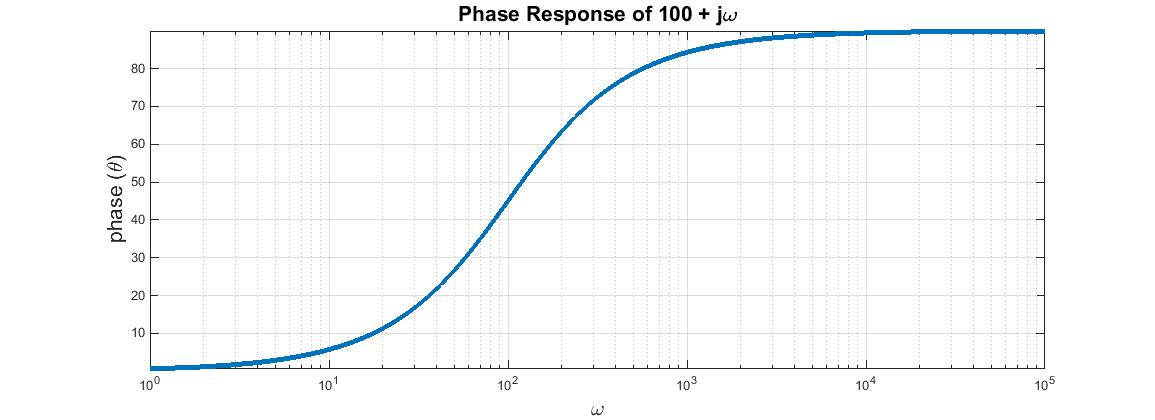
\includegraphics[width=1\textwidth]{PhaseResponse1.jpg}
\caption{A simple phase response plotted on a semilog (x) scale}
\label{fig: PhaseResponse1}
\end{figure}

Next let's plot the phase response of $\frac{200}{j\omega +50}$
\begin{figure} [h!]
\centering
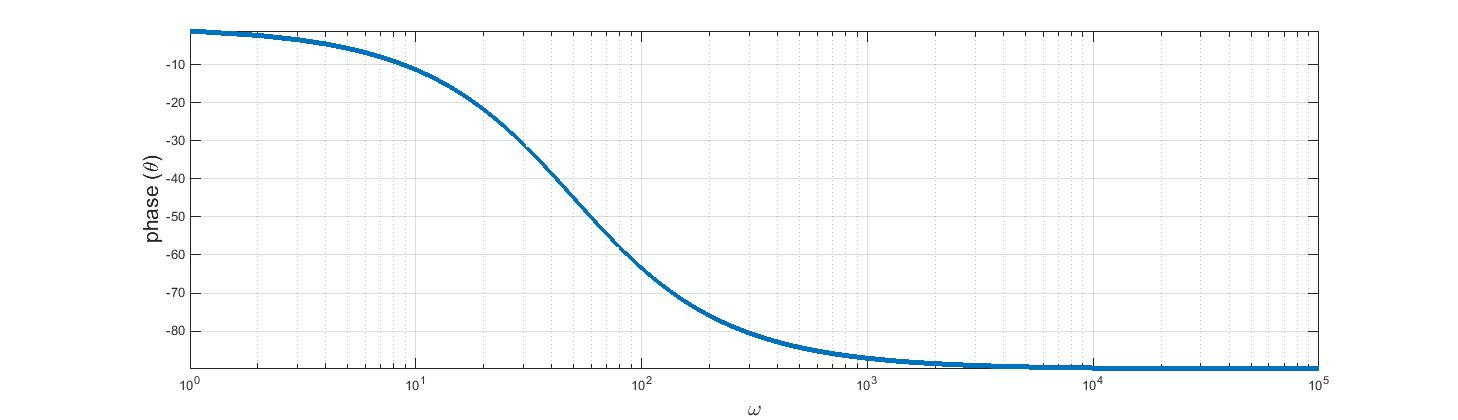
\includegraphics[width=1\textwidth]{PhaseResponse2.jpg}
\caption{A simple phase response plotted on a semilog (x) scale}
\label{fig: PhaseResponse2}
\end{figure}
\newpage
\clearpage
\pagebreak
\section{Transfer Functions}
Now that we have developed some knowledge of magnitude and phase responses and their plots, we are going to look at some circuits and develop tranfer functions.  The transfer function can be thought of as a complex gain:
\[
H(j\omega)=\frac{V_{out}(j\omega)}{V_{in}(j\omega)}
\]

\textbf{Example 1}--To demonstrate this idea lets find the transfer fucntion of the circuit in Figure \ref{fig: TransferFunction}.  Assume $C = 1\mu F$  and $R = 1k\Omega$
\begin{figure} [h!]
\centering
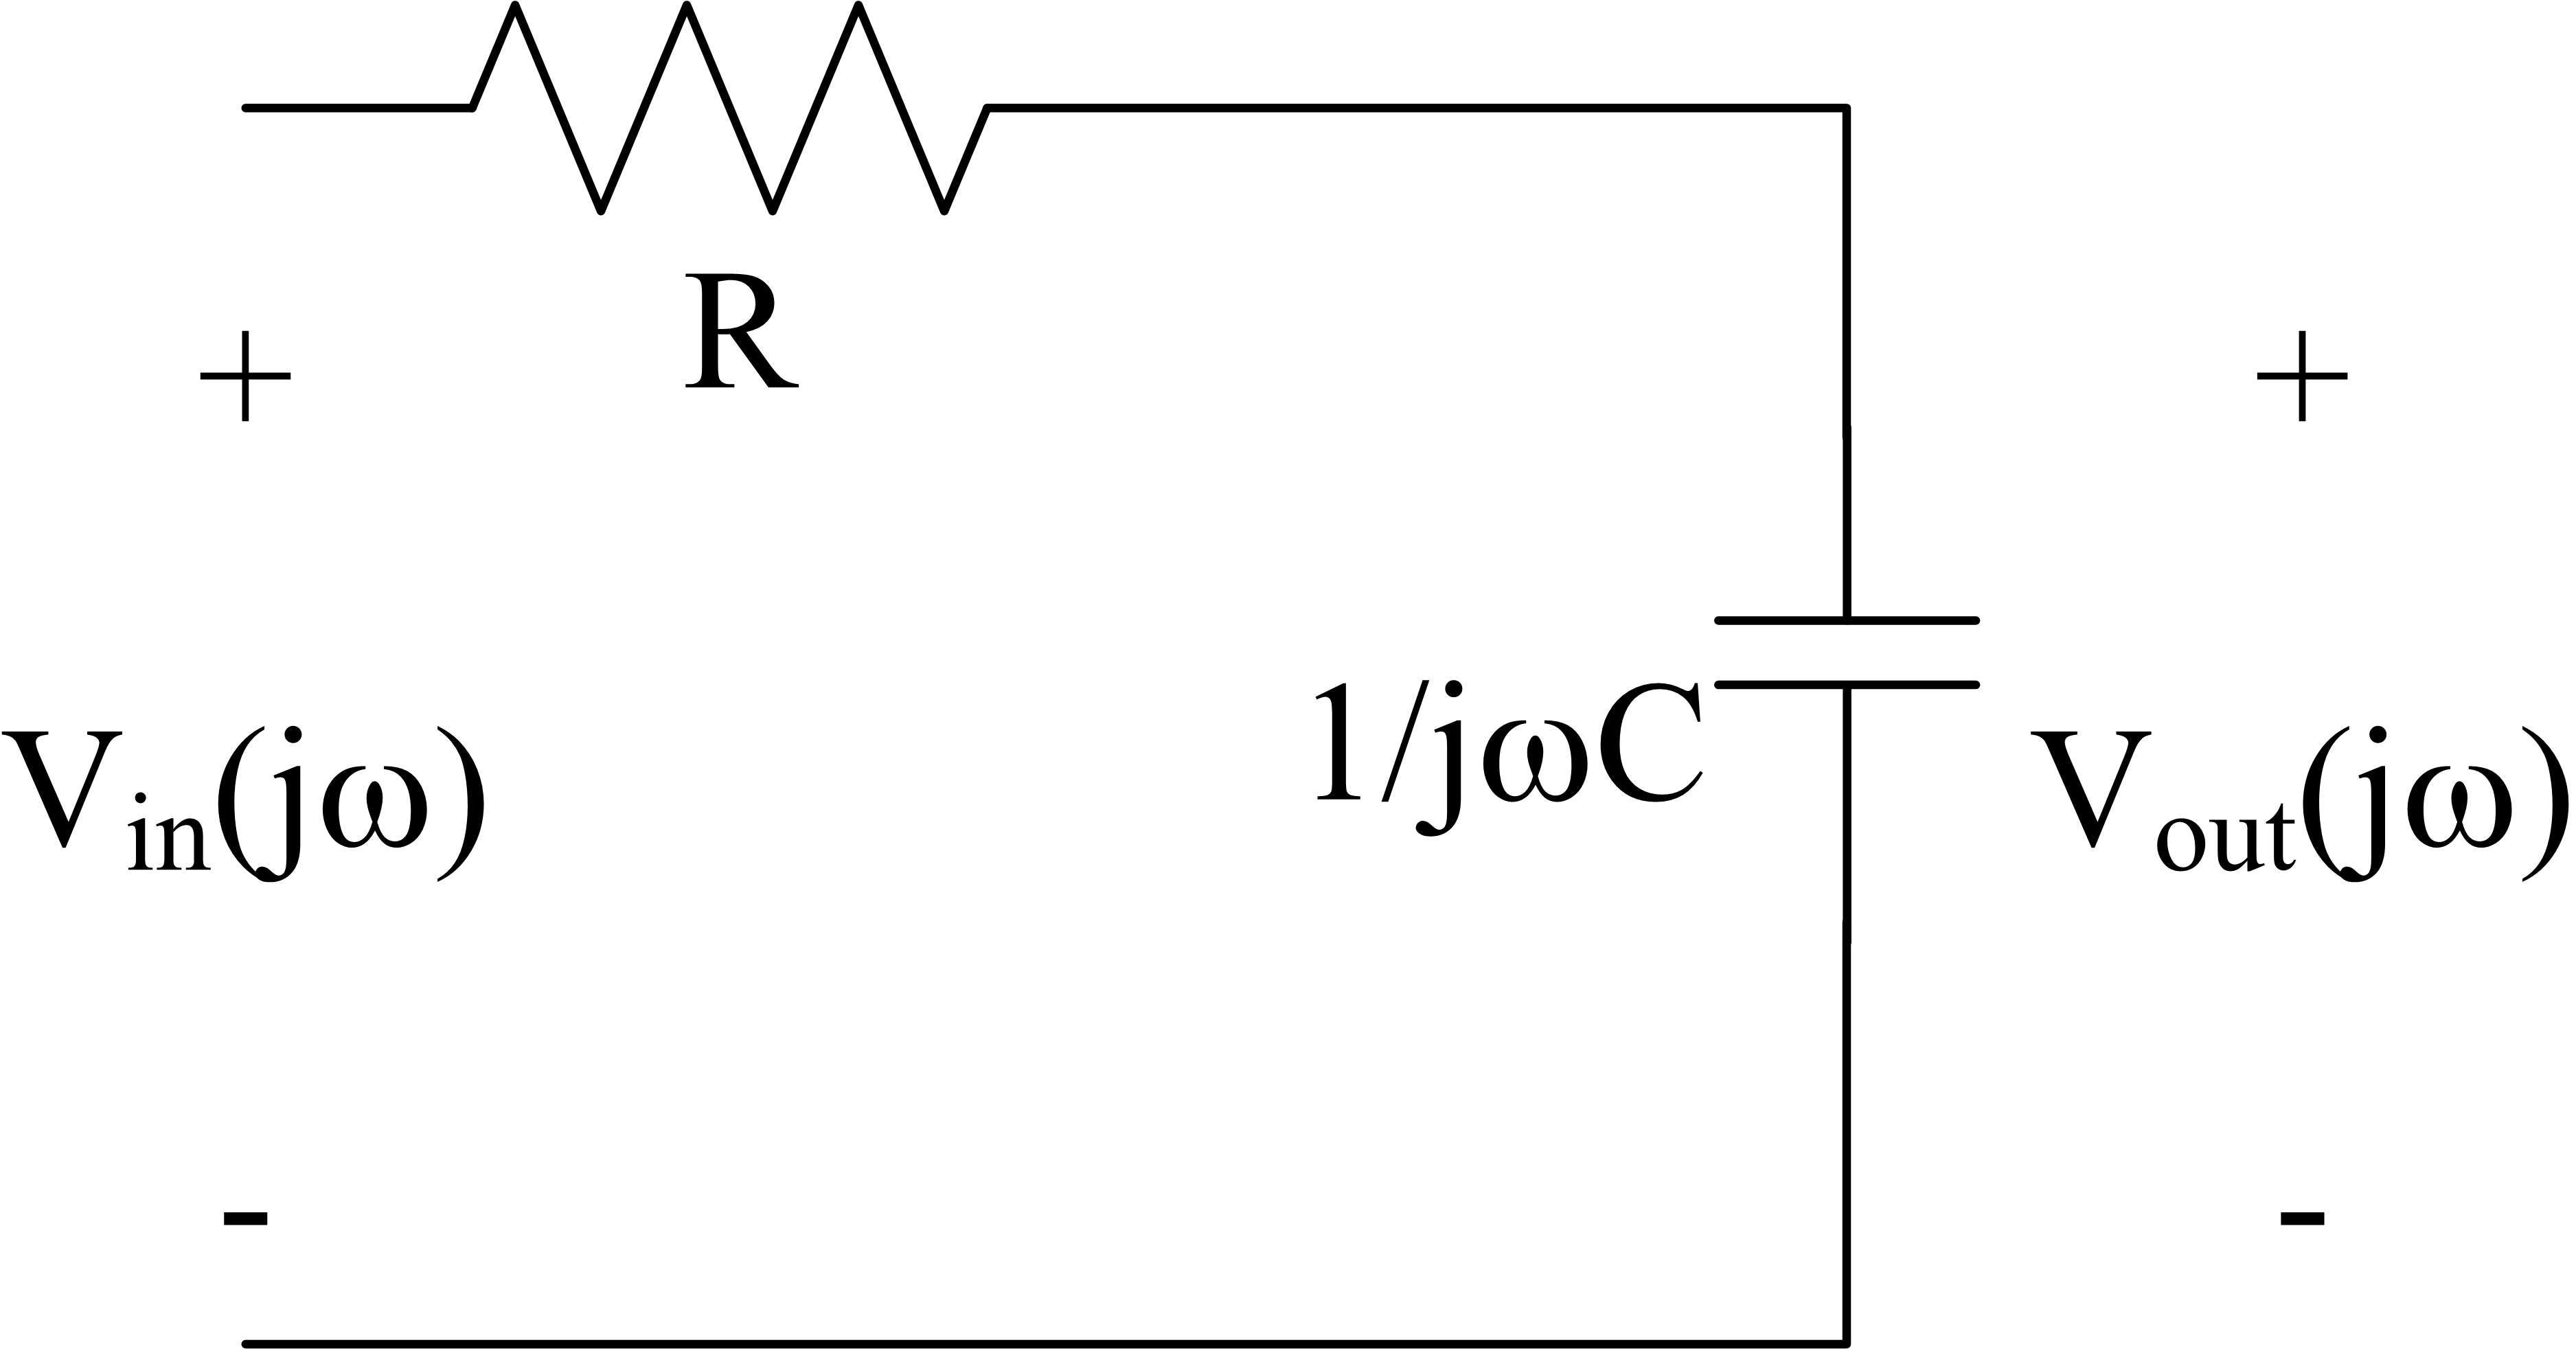
\includegraphics[width=0.3\textwidth]{TransferFunction.jpg}
\caption{Circuit to accompany Example 1}
\label{fig: TransferFunction}
\end{figure}

\soln{4in}{
We can find $V_{out}$ by doing the following voltage division
\[
V_{out}(j\omega) = V_{in}(j\omega)\frac{\frac{1}{j\omega C}}{R+\frac{1}{j \omega C}}
\]
but we need to manipulate this to get a standard form
\[
\frac{V_{out}(j\omega)}{V_{in}(j\omega)}=\frac{\frac{1}{RC}}{j\omega+\frac{1}{RC}}
\]
Now we plug infor $R$ and $C$ to get our final transfer function:
\[
\frac{V_{out}(j\omega)}{V_{in}(j\omega)}=\frac{1000}{j\omega+1000}
\]
Now we plot magnitude and phase:
\begin{figure} [h!]
\centering
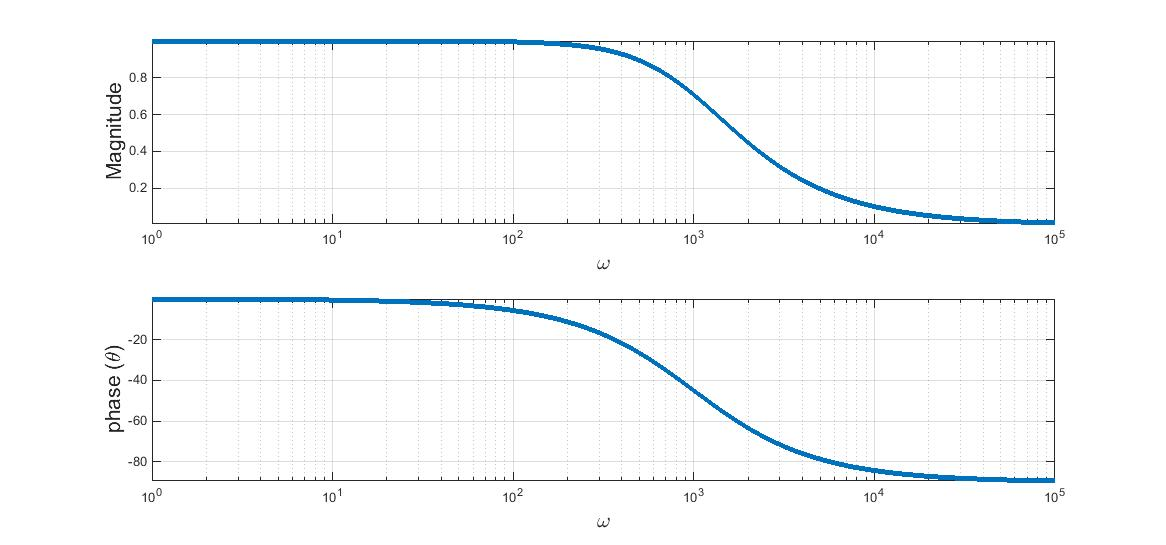
\includegraphics[width=0.9\textwidth]{TransferFunctionPlots.jpg}
\end{figure}
}


\newpage
\clearpage
\pagebreak

\textbf{Example 2} -- Write a transfer function for the circuit in Figure \ref{fig: Example2} and then plot the magnitude and phase responses given $C_{in}=500nF$, $R_{in} =1k\Omega$, $C_f=1\mu F$, and $R_f=1k\Omega$.
\begin{figure} [h!]
\centering
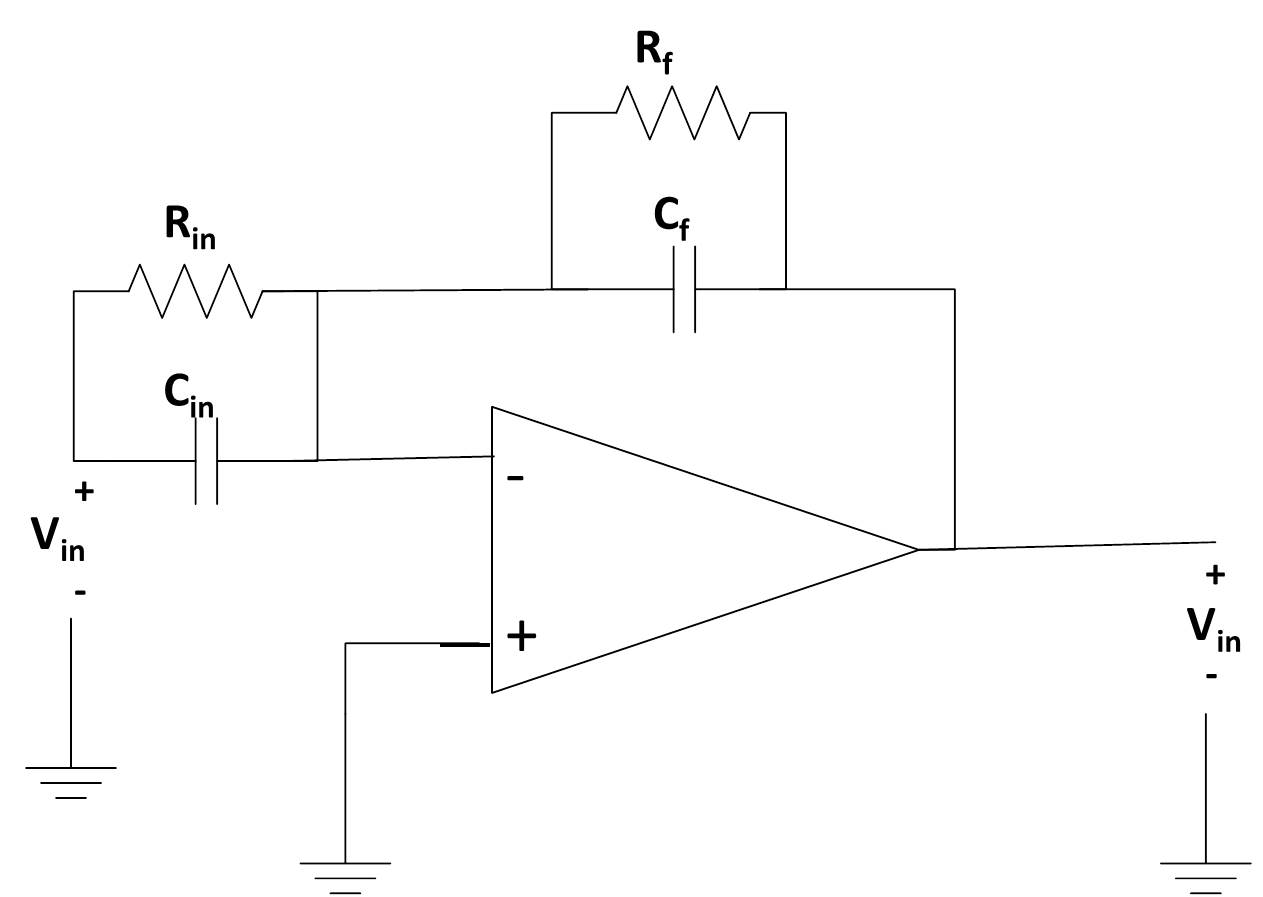
\includegraphics[width=0.6\textwidth]{Example2.jpg}
\caption{Circuit to accompany Example 2}
\label{fig: Example2}
\end{figure}

\soln{4in}{
\begin{figure} [h!]
\centering
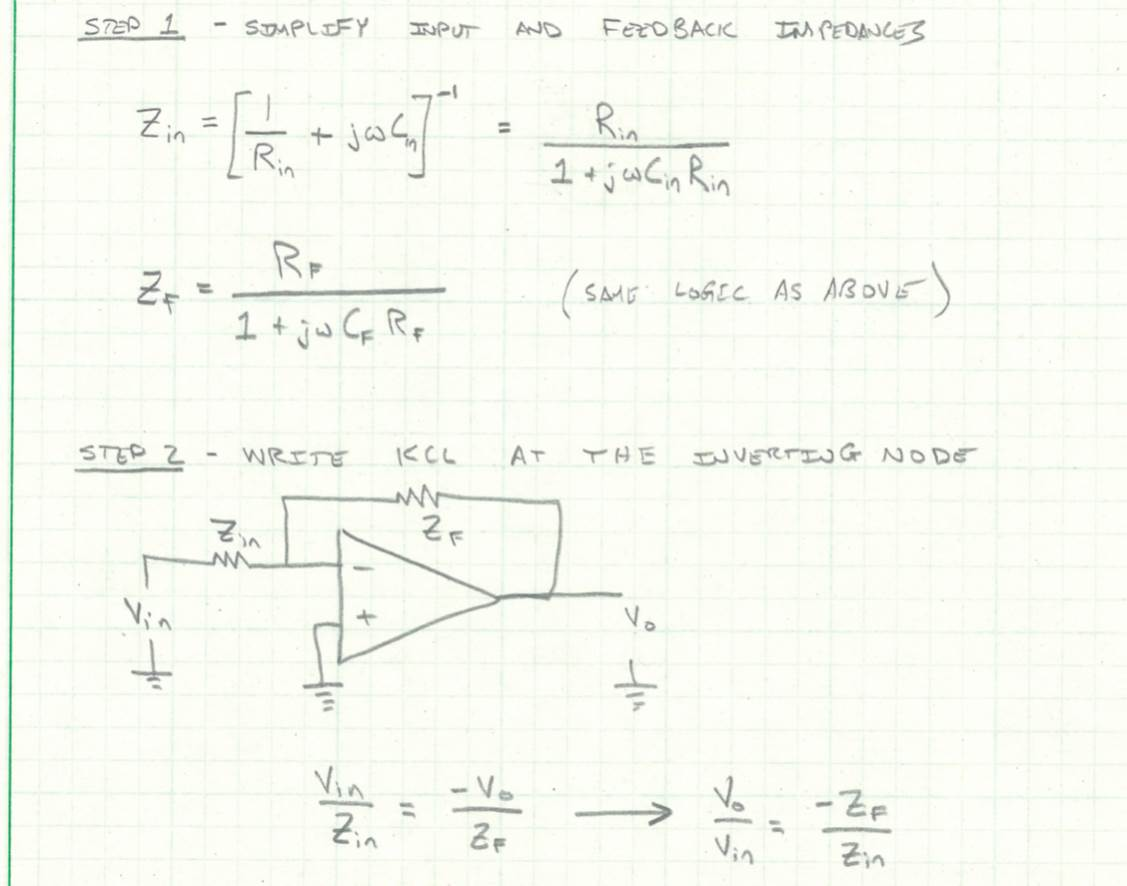
\includegraphics[width=0.9\textwidth]{Example2solnA.jpg}
\end{figure}
\begin{figure} [h!]
\centering
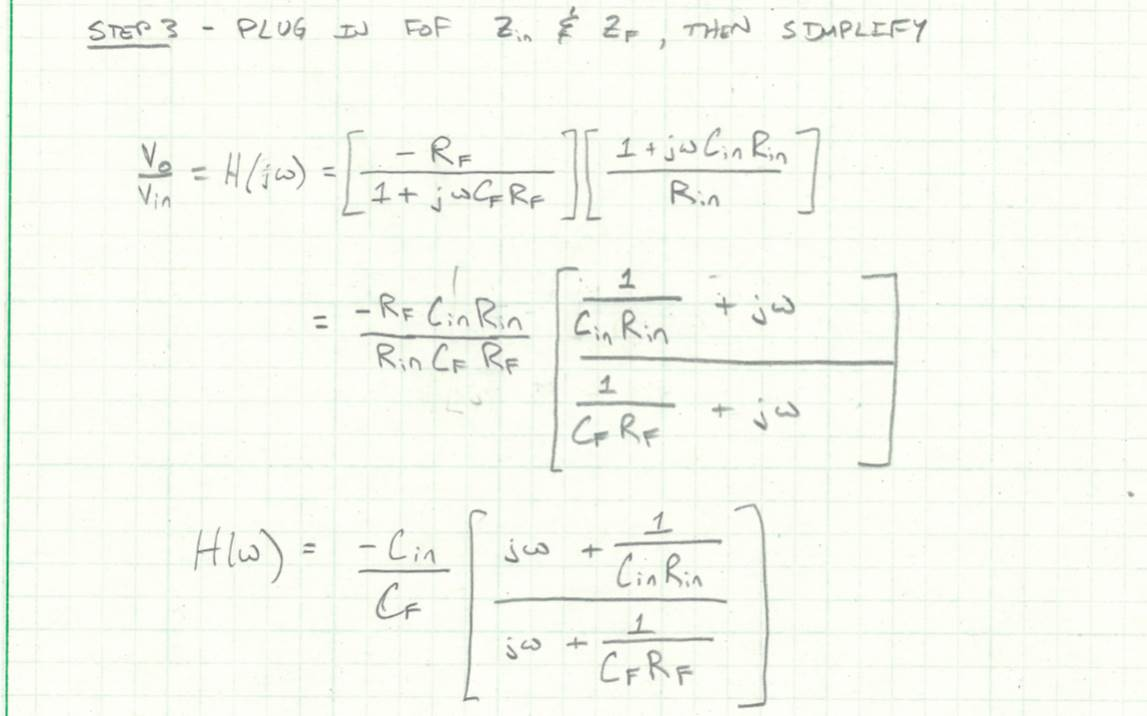
\includegraphics[width=1\textwidth]{Example2solnB.jpg}
\end{figure}
\begin{figure} [h!]
\centering
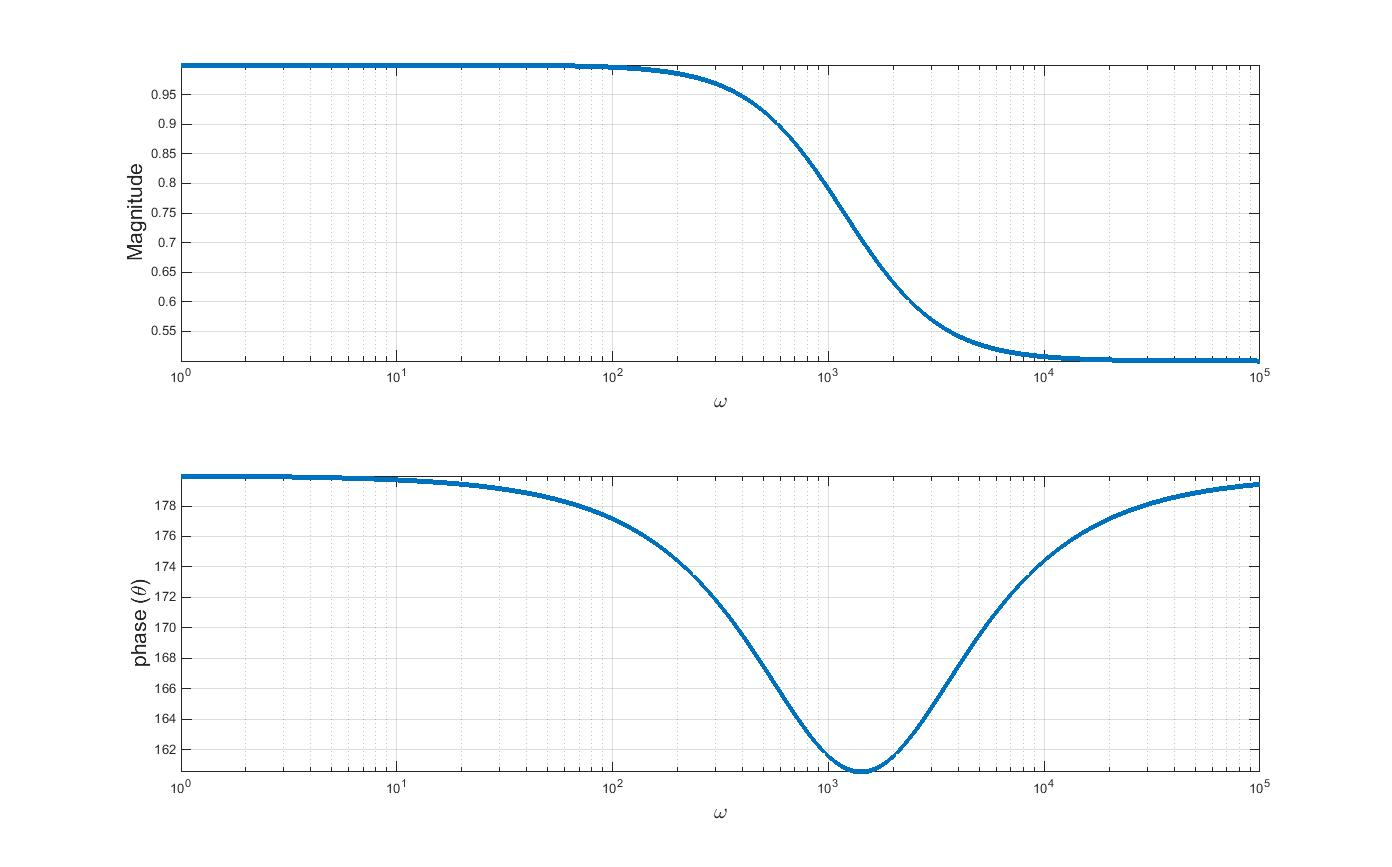
\includegraphics[width=1\textwidth]{Example2solnC.jpg}
\end{figure}
}

\newpage
\clearpage
\pagebreak

\section{Cascading Transfer Functions}
Recall all of our lessons on Op Amps where we showed we could cascade gains.  Since transfer functions are just complex gains we can cascade them as well.  The primary difference is with Op Amps your first stage could suffer from loading problems, but in general, successive stages were immune to loading; this is not the case for transfer functions in general.  In general, any stage can have loading issues when transfer functions are cascaded, but this is easily fixed with our old friend the buffer.

\textbf{Example 3}-- For the circuits in Figures \ref{fig: Example3a}, \ref{fig: Example3b}, and \ref{fig: Example3c}, find the transfer functions if $C_1=C_2$ and $R_1=R_2$.  Does the cascade (or chain) rule work as you would expect? Plot Magnitude and Phase response of each transfer function for $C_1=C_2=1\mu F$and $R_1=R_2=1k\Omega$.

\begin{figure} [h!]
\centering
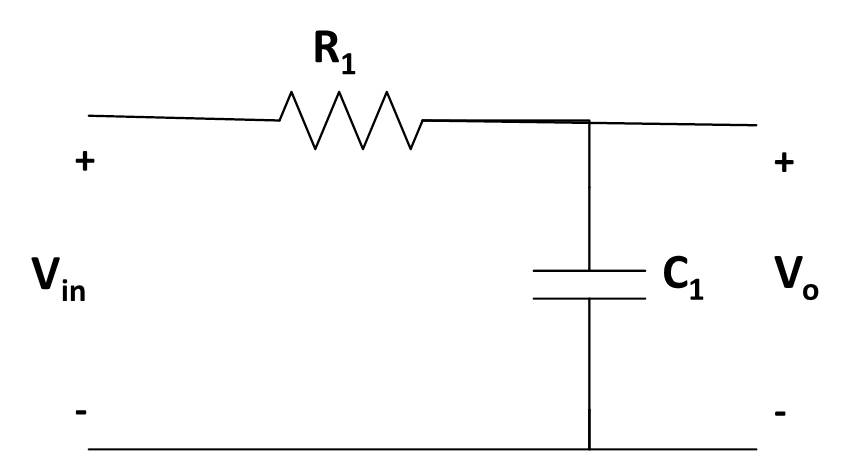
\includegraphics[width=0.4\textwidth]{Example3a.jpg}
\caption{Circuit 1 to accompany Example 3}
\label{fig: Example3a}
\end{figure}
\begin{figure} [h!]
\centering
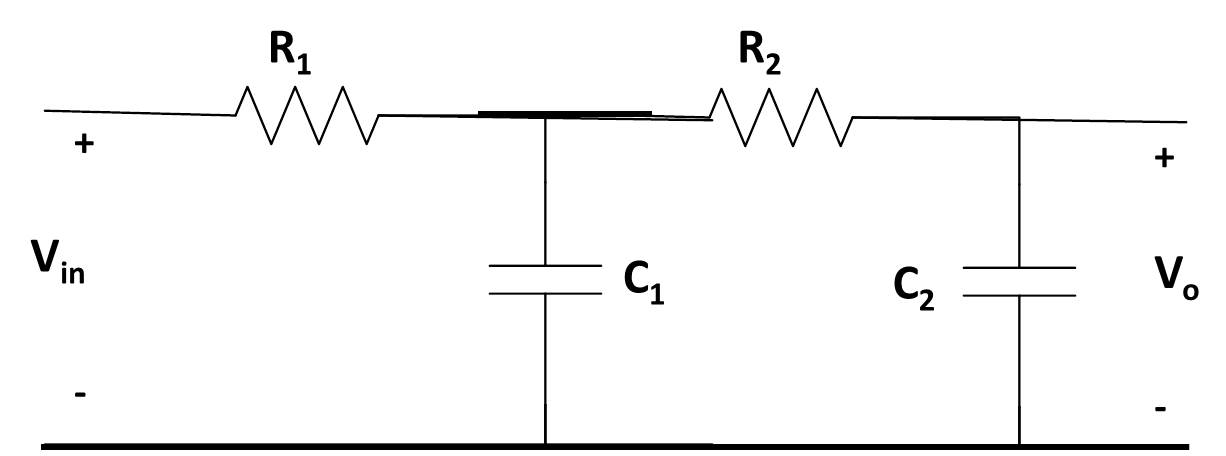
\includegraphics[width=0.6\textwidth]{Example3b.jpg}
\caption{Circuit 2 to accompany Example 3}
\label{fig: Example3b}
\end{figure}
\begin{figure} [h!]
\centering
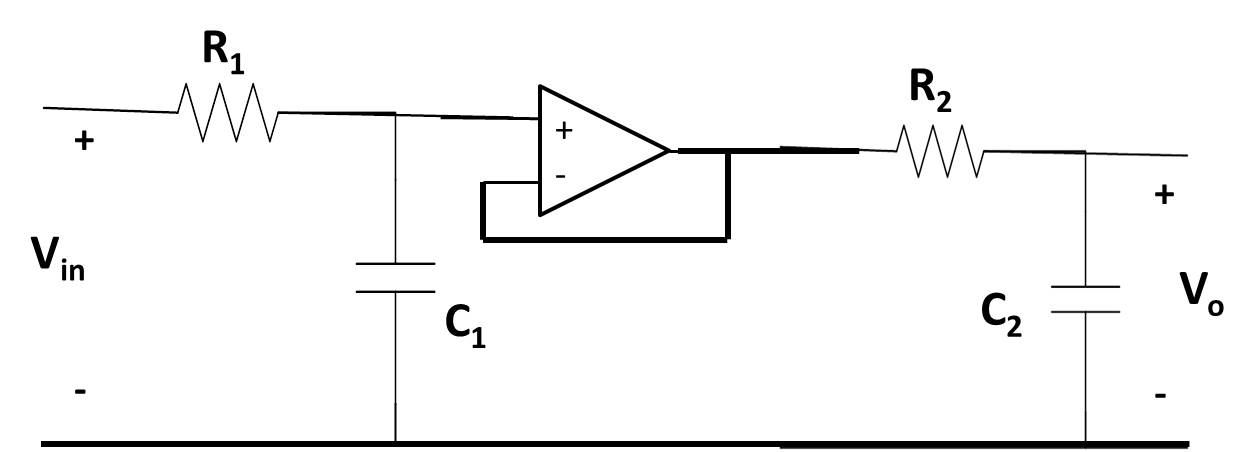
\includegraphics[width=0.6\textwidth]{Example3c.jpg}
\caption{Circuit 3 to accompany Example 3}
\label{fig: Example3c}
\end{figure}

\soln{4in}{
\begin{figure} [h!]
\centering
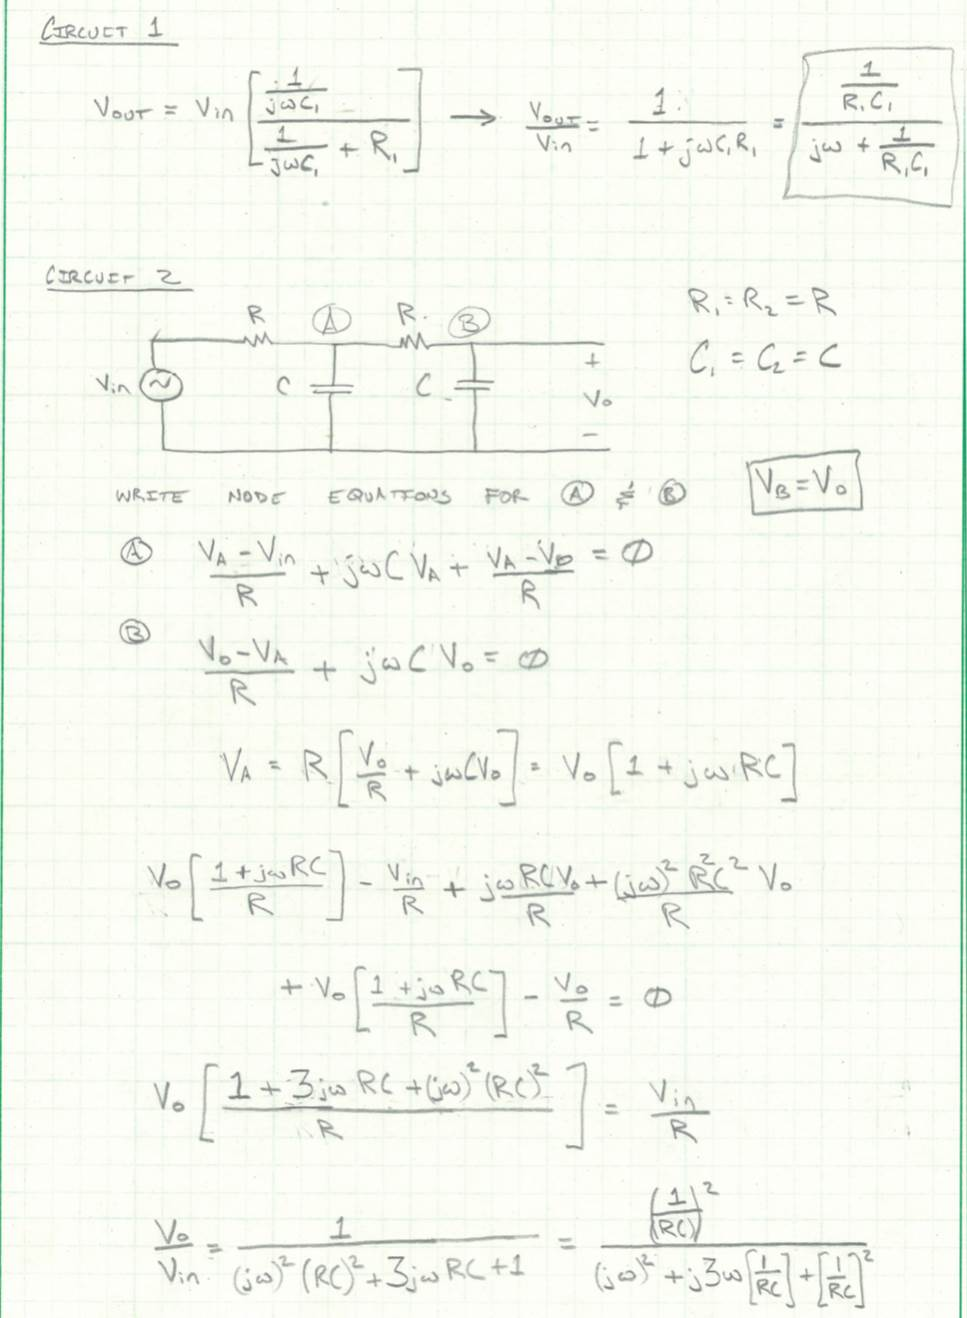
\includegraphics[width=0.9\textwidth]{Example3solnA.jpg}
\end{figure}
\begin{figure} [h!]
\centering
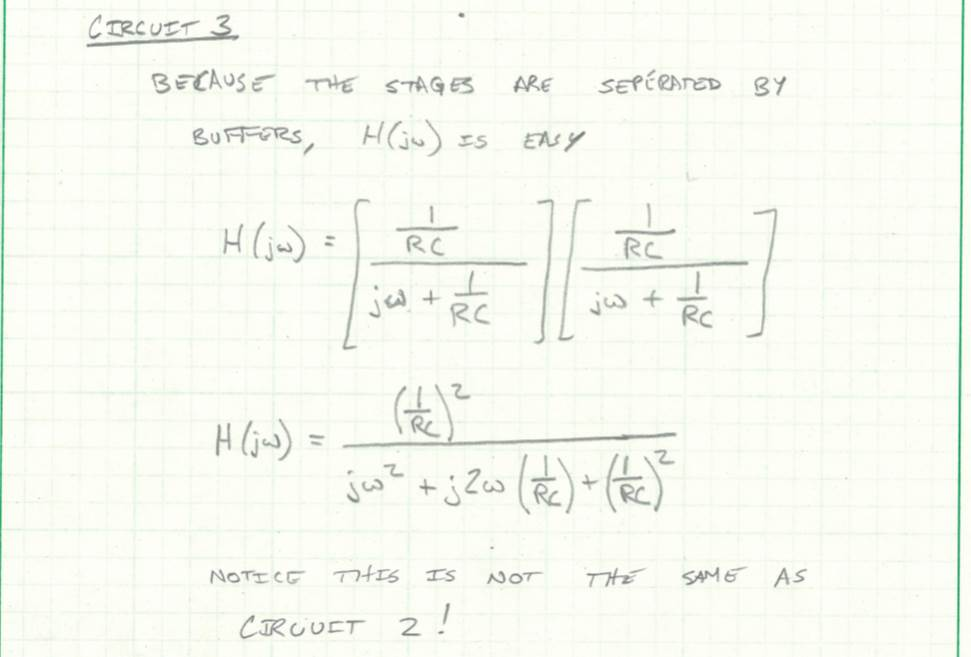
\includegraphics[width=1\textwidth]{Example3solnB.jpg}
\end{figure}
\begin{figure} [h!]
\centering
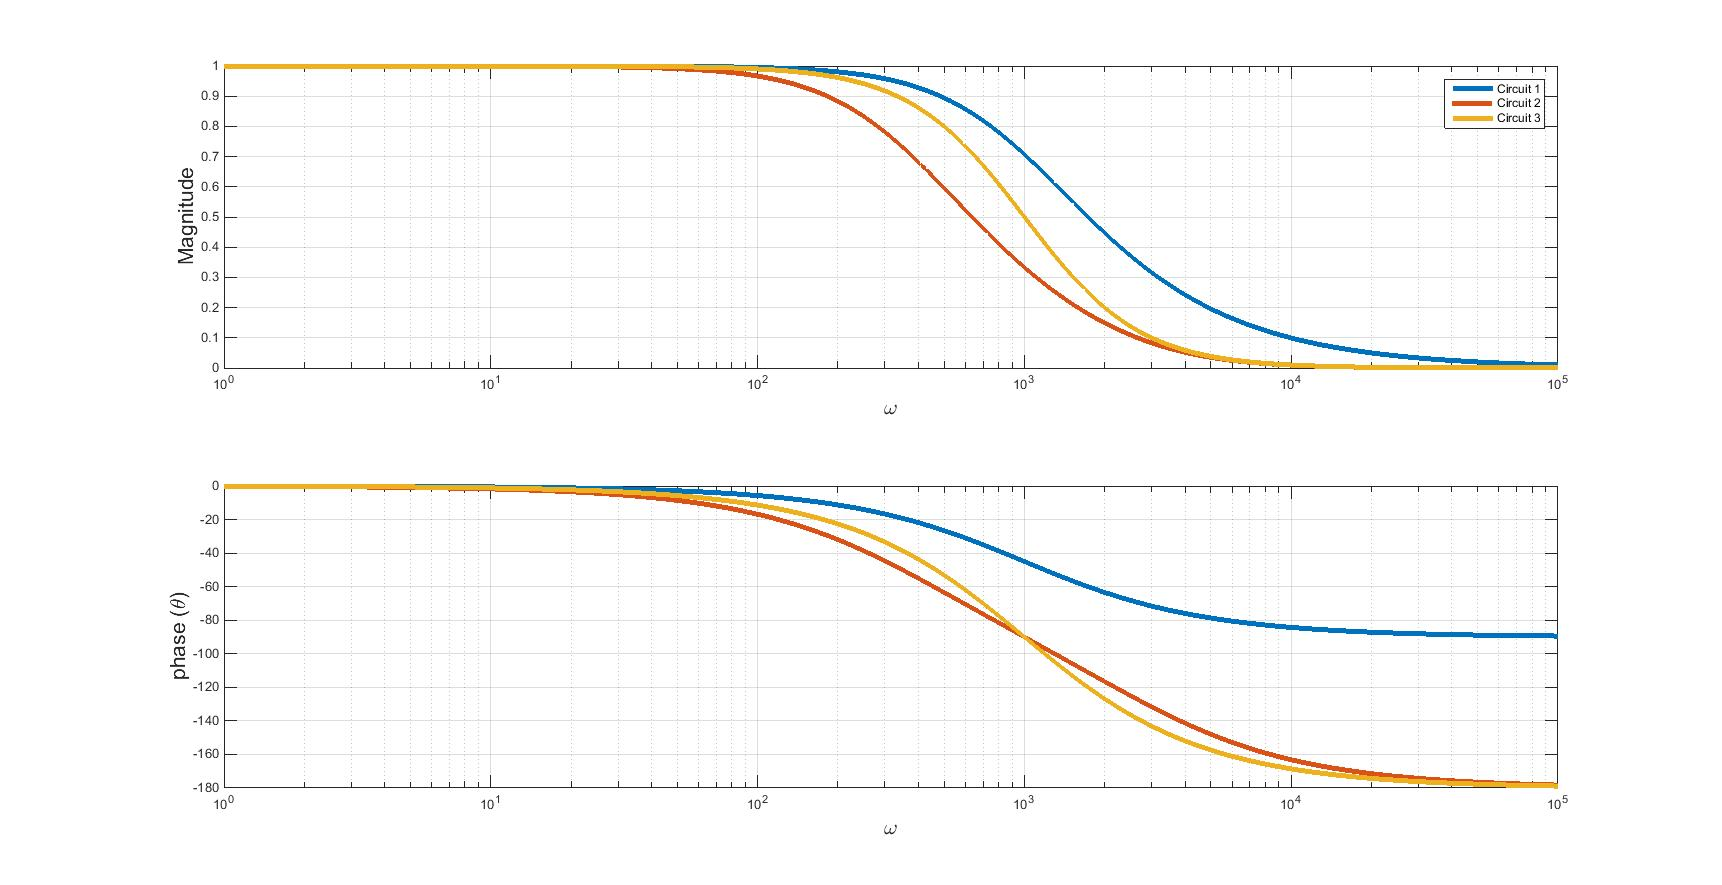
\includegraphics[width=1\textwidth]{Example3solnC.jpg}
\end{figure}
}

\end{document}


% Equation Array Example Code
%\begin
%{eqnarray}
%P_R &=& i_R^2R \nonumber \\
%P_R &=& (100\ mA)^2 \times 100\ \Omega \nonumber \\
%P_R &=& (100 \times 10^{-3}\ A)^2 \times 100\ \Omega \\
%P_R &=& 10000 \times 10^{-6}\ A^2  \times 100\ \Omega \nonumber \\
%P_R &=& 1\ W  \nonumber
%\end{eqnarray} 

% Figure Example Code
%\begin{figure} [h!]
%\centering
%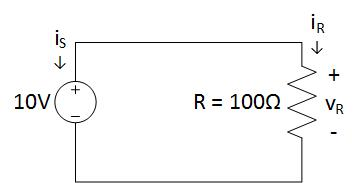
\includegraphics[width=0.5\textwidth]{OhmsLawExampleSolution.jpg}
%\caption{Ohm's Law example circuit}
%\label{fig: OhmsLawExampleSolution}
%\end{figure}

%Table Example Code
%\begin{table}[h]
%\centering
%\begin{tabular}{|l|c|c|}
%\hline
%Prefix & Abbreviation & Value \\
%\hline \hline
%Giga & $G$ & $10^9$ \\
%Mega & $M$ & $10^6$ \\
%Kilo & $k$ & $10^3$ \\
%\hline
%milli & $m$ & $10^{-3}$ \\
%micro & $\mu$ & $10^{-6}$ \\
%nano & $n$ & $10^{-9}$ \\
%pico & $p$ & $10^{-12}$ \\
%\hline
%\end{tabular}
%\caption{Engineering prefixes and values}
%\label{tab: Eng Prefixes}
%\end{table}
